\selectlanguage{english}%

\chapter{Implementação} \label{capImp}
A implementação em bancada inicia-se com a calibração dos sensores, uma vez que o comportamento observado no sistema real parece não manter suas configurações dia a dia. Em seguida, realiza-se a identificação dos ganhos das bombas e do sistema em 4 pontos, que irão compor os conjuntos fuzzy TS. Por fim, os ganhos são calculados seguindo as \jhhref{eqContFuzzy}{equações} e aplicados utilizando os procedimentos demonstrados a seguir.

\section{Identificação}
Inicialmente, tentou-se realizar a identificação do sistema utilizando algoritmos computacionais, como a Toolbox de Identificação do Matlab. Para isso foram realizadas várias testes de entrada e saída no sistema:
\begin{figure}[H]
	\centering
	\begin{tabular}{cc}
		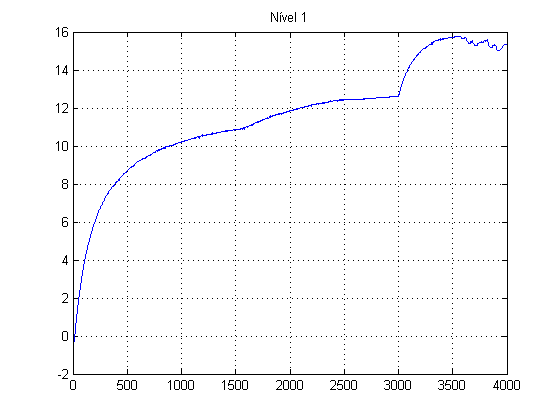
\includegraphics[height=0.2\paperheight,keepaspectratio]{img/sim1_h1.png} &
		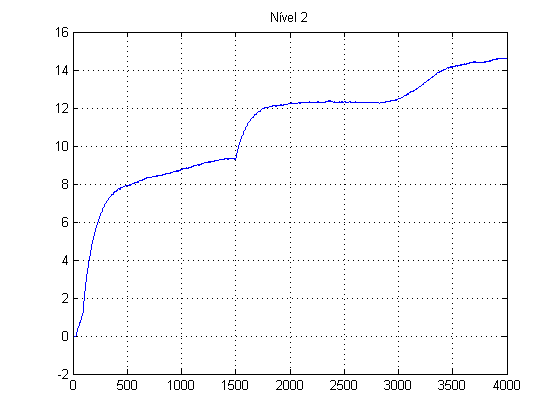
\includegraphics[height=0.2\paperheight,keepaspectratio]{img/sim1_h2.png} \\
		(a) Nível 1 &
		(b) Nível 2 \\
		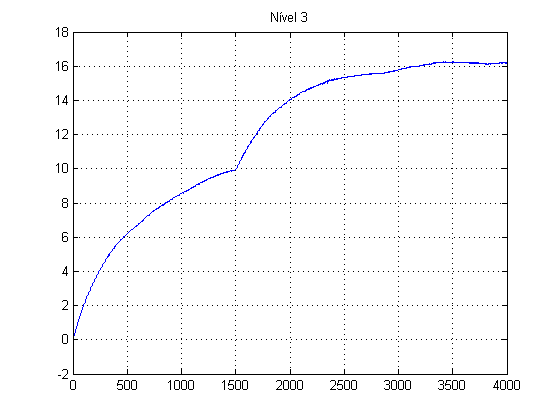
\includegraphics[height=0.2\paperheight,keepaspectratio]{img/sim1_h3.png} &
		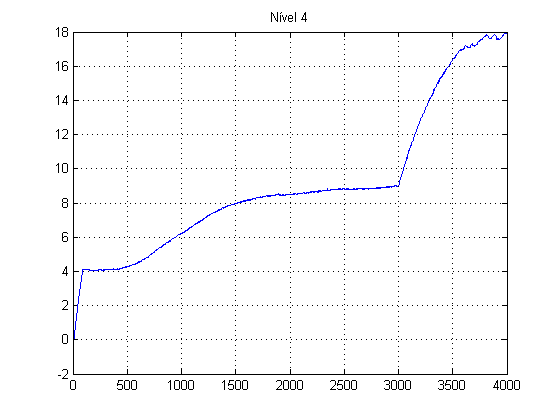
\includegraphics[height=0.2\paperheight,keepaspectratio]{img/sim1_h4.png} \\
		(c) Nível 3 &
		(d) Nível 4
	\end{tabular}
	\caption{\label{imgID_4000} Identificação 1 - 4000 segundos}
\end{figure}

\begin{figure}[H]
	\centering
	\begin{tabular}{cc}
		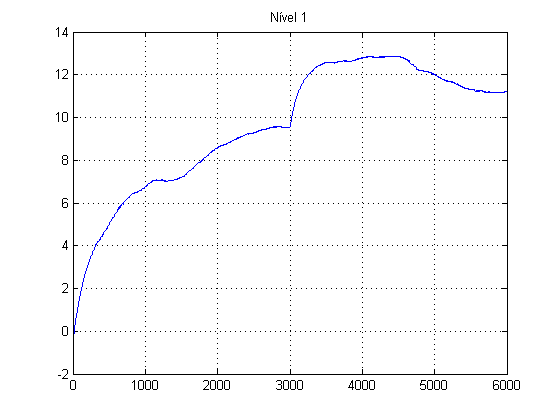
\includegraphics[height=0.15\paperheight,keepaspectratio]{img/sim2_h1.png} &
		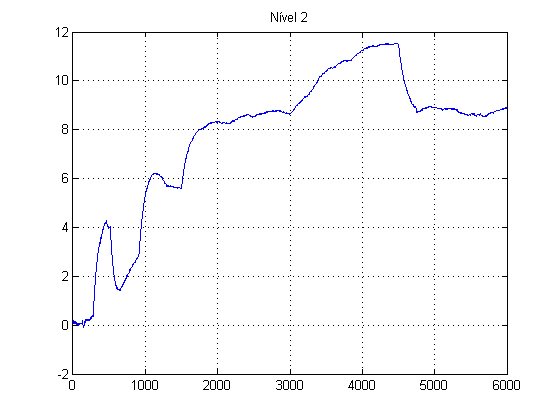
\includegraphics[height=0.15\paperheight,keepaspectratio]{img/sim2_h2.png} \\
		(a) Nível 1 &
		(b) Nível 2 \\
		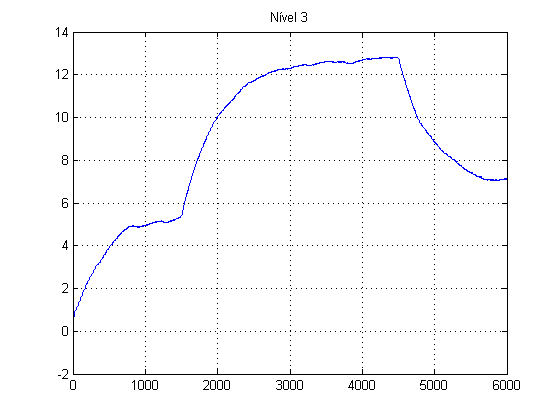
\includegraphics[height=0.15\paperheight,keepaspectratio]{img/sim2_h3.png} &
		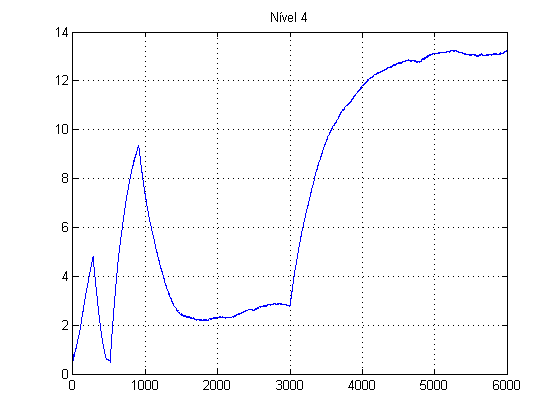
\includegraphics[height=0.15\paperheight,keepaspectratio]{img/sim2_h4.png} \\
		(c) Nível 3 &
		(d) Nível 4
	\end{tabular}
	\caption{\label{imgID_4500} Identificação 2 - 4500 segundos}
\end{figure}

\begin{figure}[H]
	\centering
	\begin{tabular}{cc}
		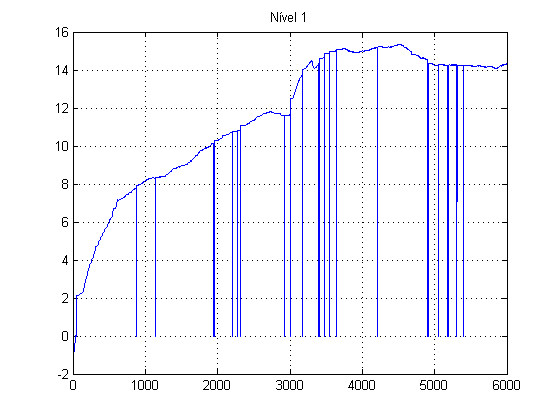
\includegraphics[height=0.15\paperheight,keepaspectratio]{img/sim3_h1.png} &
		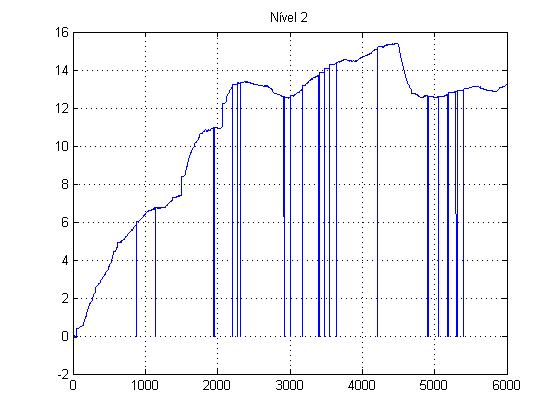
\includegraphics[height=0.15\paperheight,keepaspectratio]{img/sim3_h2.png} \\
		(a) Nível 1 &
		(b) Nível 2 \\
		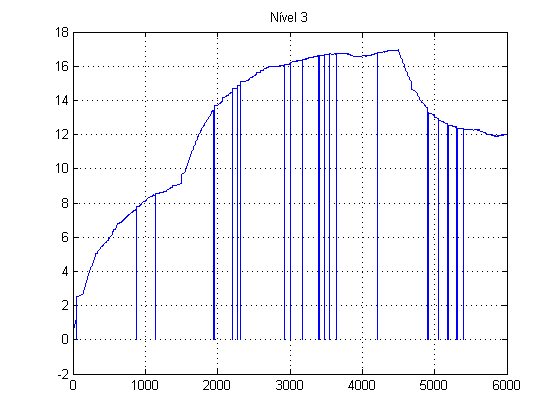
\includegraphics[height=0.15\paperheight,keepaspectratio]{img/sim3_h3.png} &
		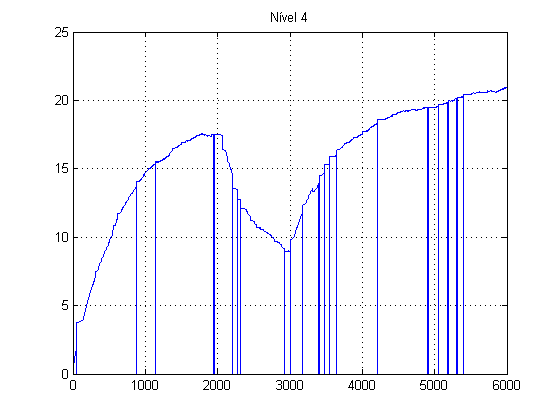
\includegraphics[height=0.15\paperheight,keepaspectratio]{img/sim3_h4.png} \\
		(c) Nível 3 &
		(d) Nível 4
	\end{tabular}
	\caption{\label{imgID_6000} Identificação 3 - 6000 segundos}
\end{figure}

No entanto, apesar de encontrar modelos que se encaixavam bem as curvas, os resultados obtidos por este método não eram nada condizentes com a dinâmica já conhecida e os ganhos obtidos foram muito esdrúxulos.

Optou-se então por realizar manualmente a identificação do sistema. Ao enviar degraus de entrada e observando as respostas em regime permanente, em conjunto com os parâmetros conhecidos da planta, torna-se possível a identificação de um modelo condizente ao esperado e muito eficiente localmente, o que é desejado na modelagem TS.

Escolheu-se realizar-se a identificação para o funcionamento das bombas a 42\% e 45\% de suas capacidades. Nota-se que abaixo de 30\% não há resposta aparente e durante todo este trabalho limitou-se a atuar abaixo de 70\% de sua potência máxima, uma vez que este valor foi observado como limiar seguro de utilização.

\begin{center} \label{tabIdentKs}
	\begin{tabular}{|c|c|c|c|c|c|c|}
		\hline
		Identificação & Tensão ($v_i$)&  $\gamma_1$ & $\gamma_2$ & Ganho 1 ($k_1$) & Ganho 2 ($k_2$) \\ \hline
		1 & 42\% & 0.8980 & 0.6810 & 7.4044 $cm^3/Vs$ & 7.1022 $cm^3/Vs$\\ \hline
		2 & 45\% & 0.8276 & 0.6827 & 8.1801 $cm^3/Vs$ & 7.3339 $cm^3/Vs$\\ \hline
	\end{tabular}
\end{center}

Realiza-se então a identificação do modelo, a partir dos estados estacionários, nos 4 pontos dados pela interpolação destes conjuntos. Os resultados obtidos são exibidos a seguir:

\begin{center}
	\begin{tabular}{|c|c|c|c|c|c|c|}
		\hline
		Sistema & Bomba 1 ($\bar{v_1}$) & Bomba 2 ($\bar{v_1}$) & Nível 1 ($\bar{h_1}$) & Nível 2 ($\bar{h_2}$) & Nível 3 ($\bar{h_3}$) & Nível 4 ($\bar{h_4}$) \\ \hline
		1 & 42\% & 42\% & 11.1024 cm &  9.4410 cm &  8.7849 cm & 17.4466 cm \\ \hline
		2 & 42\% & 45\% & 16.3767 cm &  16.1350 cm & 11.4907 cm & 20.5671 cm \\ \hline
		3 & 45\% & 42\% & 15.0037 cm &  13.9138 cm & 20.7899 cm & 19.5759 cm \\ \hline
		4 & 45\% & 45\% & 18.0278 cm &  18.8761 cm & 18.3048 cm & 19.6136 cm \\	\hline
	\end{tabular}
\end{center}

São obtidas então 4 regras e para cada uma delas um controlador, sintonizado seguindo as \jhhref{eqContFuzzy}{equações}. A tabela a seguir apresenta os ganhos obtidos:
\begin{center} \label{tabGanhosReais}
	\begin{tabular}{|c|c|}
		\hline
		Regra & Ganho \\ \hline
		1 & $ K = 
		\begin{bmatrix}
			-10.1267 &  -0.1726 & -0.0693 &  -0.0304 & 7.4632  &  0.0782 \\
			0.4704   & -8.9962  &  0.0234 &  -0.0081 & -0.1735 & 11.3821
		\end{bmatrix}$ \\[10pt] \hline
		2 & $ K = 
		\begin{bmatrix}
			-10.1655 &  -0.1445 &  -0.0628 &  -0.0301 &  7.4634 & 0.0680 \\
			0.3944   & -8.7470  &  0.0221  & -0.0071  & -0.1460 & 11.0130
		\end{bmatrix}$ \\[10pt] \hline
		3 & $ K = 
		\begin{bmatrix}
			-9.7178 &  -0.2288 &  -0.0433 &  -0.0878 &   7.1828 &   0.0979 \\
			0.5970  & -8.9866  & -0.0014  & -0.0096  & -0.2192  & 11.3719
		\end{bmatrix}$ \\[10pt] \hline
		4 & $ K = 
		\begin{bmatrix}
			-9.7327 &  -0.2180 &  -0.0472 &  -0.0874 &   7.1831 &   0.0939 \\
			0.5519  & -8.7291  &  0.0082  & -0.0090  & -0.2028  & 11.0068
		\end{bmatrix}$ \\[10pt] \hline
	\end{tabular}
\end{center}

\section{CLP}
Os ganhos obtidos a partir da identificação do modelo foram implementados no CLP utilizando um diagrama de bloco de funções e uma rotina em texto estruturado. A \jhhref{figCLPCLPbf}{Figura} a seguir apresenta o programa principal. 

\begin{figure}[H]
	\centering
	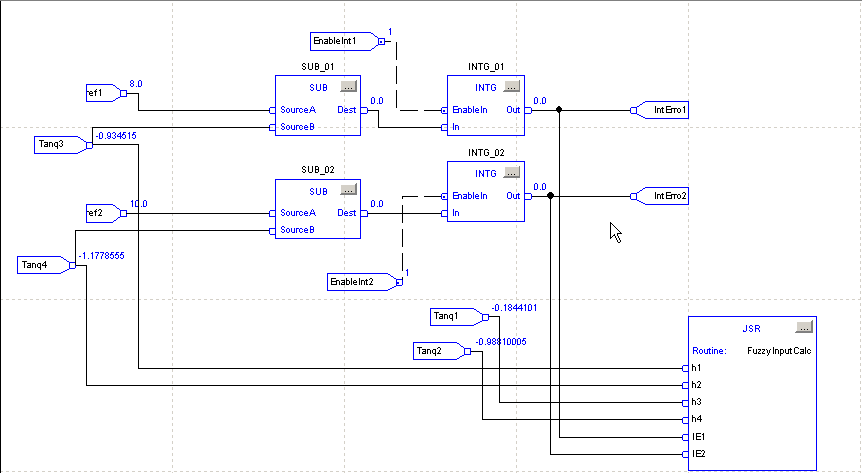
\includegraphics[width=\textwidth]{img/clp_bf2.png}
	\caption{Programa Principal}
	\label{figCLPCLPbf}
\end{figure}

O controlador recebe os estados atuais do sistema e os erros acumulados das variáveis controladas. A rotina textit{FuzzyInputCalc} implementa o controlador fuzzy a partir destas entradas e dos ganhos já apresentados assinalando às variáveis de saída o valor da tensão nas bombas desejado. A \jhhref{figCLPTags1}{Figura} a seguir apresenta as variáveis definidas no trabalho.

\begin{figure}[H]
	\centering
	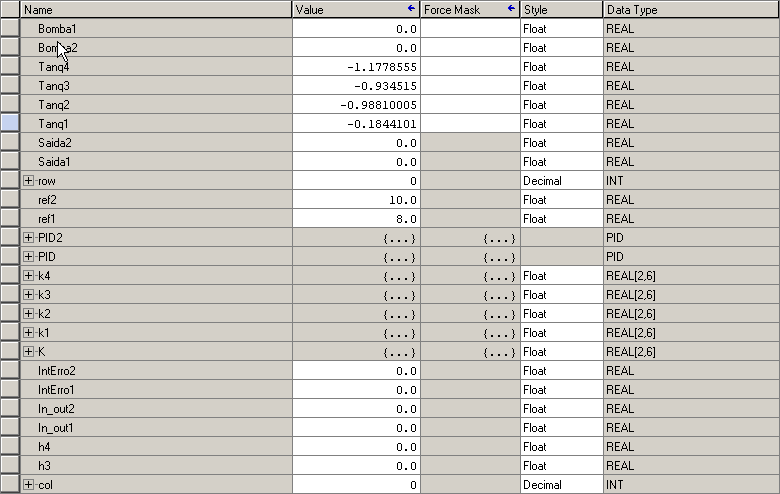
\includegraphics[width=0.7\textwidth]{img/tags1.png}\\
	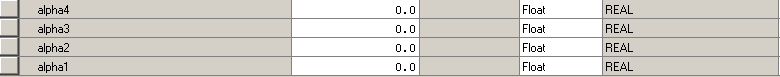
\includegraphics[width=0.7\textwidth]{img/tags2.png}
	\caption{Variáveis do programa}
	\label{figCLPTags1}
\end{figure}

Os resultados obtidos são apresentados na \jhhref{secResImp}{seção} a seguir.

\selectlanguage{brazil}%

